\chapter{LMGesture library dedicated for Leap Motion controller}

\section{Architecture}

\subsection{Model}

While data from the LMR files are being processed, they are stored using a specially created class representing the data. GestureFrame represents a single frame obtained from Leap Motion Controller. All gathered data is stored in a vector containing elements of GestureFrame type. GestureFrame holds information such as:

\begin{itemize}
\item timestamp,
\item list of hands occurring in the frame, stored in a vector containing elements GestureHand type.
\end{itemize}

GestureHand stores parameters of hand performing gesture. In one instance of GestureFrame can be stored many instances of GestureHand. GestureHand holds following information:
\begin{itemize}
\item hand id,
\item plam position,
\item stabilized palm position,
\item palm normal vector,
\item palm direction,
\item list of fingers of particular hand, stored in a vector containing elements GestureFinger type,
\item ordered value, obtained during hand sorting.
\end{itemize}

GestureFinger stores parameters of one finger. In one instance of GestureHand can be stored many instances of GestureFinger. GestureFinger contains:
\begin{itemize}
\item finger id,
\item tip position,
\item stabilized tip position,
\item finger direction,
\item finger length,
\item finger width,
\item ordered value, obtained during finger sorting.
\end{itemize}

\section{Processes}

\subsection{The learning process}
The learning process is a process, which shows how user can teach LMGesture library a new gesture. First  gestures must be recorded gestures in LMR format. To obtain recordings in this format user may use Gesture Recorder --  a module included in the library, which records data from Leap Mption Controller and saves it as LMR file. When all desired gestures are prepared, the user starts the process of learning by {\color{red}[tutaj dodać informacje jak uruchomić ten prces - prawdopodobnie jakas komenda + jakies parametry typu -d uczenie gestów dynamicznych, -s uczenie gestów statycznych + pliki LMR jako argumenty]}. 

\begin{figure}[htb]
\centering
 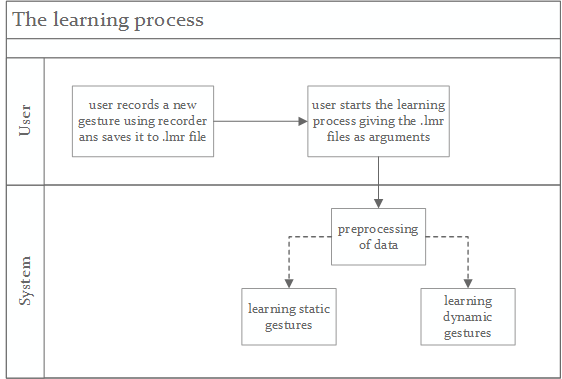
\includegraphics[width=0.75\columnwidth]{figures/learningProcess.png}
 \caption{Diagram showing the learning process}
 \label{learningprocess}
\end{figure}

The first step in the learning process, which is performed by the system is the preprocessing of data. Training data should be deprived of noise or should not have lost fingers for several frames. According to user-specified parameters, the system will learn the gesture as a static or dynamic gesture. Appropriate way of learning corresponds to the appropriate gesture.
For the learning static gesture system uses a support vector machine (SVM), and for dynamic gestures uses hidden Markov model (HMM). 
The learning process for static gestures:
\begin{enumerate}
\item In the first stage, data which will be used during the learning is preprocessed.
\item Data are scaled using internal scaling module. The result of this step are scale and range files. In the scale file scaled data is stored. The range file contains information that enables to scale any data in the same way.
\item Scale file with scaled data is transmitted to training module. Data is processed using SVM algorithm. Additionally during learning process k-validation is performed and results are returned to the user. In process model file is created, which is used during static gesture recognition process.
\end{enumerate}
{\color{red}[opisać learning process dla dynamicznych]}


\subsection{The recognition process}
The recognition process is a process in which the system attempts to match gesture given by a user, to the set of gestures obtained by the learning process. {\color{red}[Opis procesu recognition process, przedstawienie scenariusza uzycia w stosunku do architektury]}

\begin{figure}[htb]
\centering
 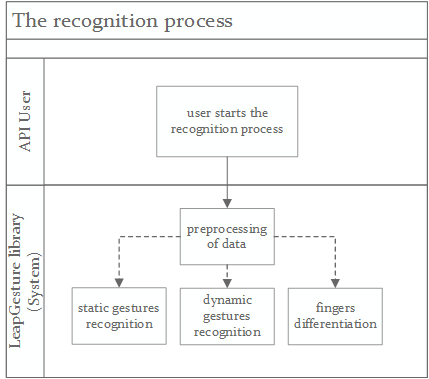
\includegraphics[width=0.6\columnwidth]{figures/recognitionProcess.png}
 \caption{Diagram showing the recognition process}
 \label{recognitionprocess}
\end{figure}

Modules handlers are implemented using the Observer pattern. For each of the modules are specified relevant events that are reported in the key moments of recognition such as: moment in which particular gesture began to be recognized, moment in which the particular gesture stopped being recognized, moment in which frame processing is finished.
The user can handle events received in specific module by implementing appropriate listener interface and adding reference to listener list in specific library module. During gesture recognition process user can use from 1 to 3 listeners. Each listener is on a separate thread.

Methods for a static gesture observer:
\begin {itemize}
\item onStart -- signals the start of the gesture,
\item onFrame -- returns a list of recognized gestures with matching probabilities,
\item onGesture -- signals the end of the gesture and returns a list of recognized gestures with matching probabilities.
\end {itemize}

Methods for a dynamic gesture observer:
\begin {itemize}
\item onStart, onFrame -- have the same purposes as in the case of static observer,
\item onGesture -- signals the end of the gesture and returns a list of recognized gestures with matching probabilities and parameter values.
\end {itemize}

Methods for a finger differentiation observer:
\begin {itemize}
\item onFrame -- returns a list of matched classes with probabilities,
\item onChange -- signals a change of fingers arrangement.
\end {itemize}

As in the learning process for recognizing static gestures system uses SVM and for dynamic gestures -- HMM. For finger differentation system uses support vector machine. However, there are other classes than those used for static gestures recogniton.

\section{Gesture recorder and visualizer}
Recorder and vizualizer module is an additional part of library that allows users for easy management of gestures recordings. The recorder collects data from Leap Motion Controller, converts it into data representation described in section regards architecture of library {\color{red}[weryfikacja po skleceniu pracy]} and writes it to the LMR file, which is supported by the LMGesture library. Visualizer enables users to see the recorded gestures stored in LMR format. Data gathered from Leap Motion, used to recognize gestures are very large and the data processed in the library have a specific format. Therefore, it was necessary to create an auxiliary program, that it would facilitate the work with data in the fastest and most user-friendly way.

\subsection{LMR files}
This is a file format specially developed for the LMGestue library, supported by various modules for example by the visualizer. The file structure is as follows:
\begin{itemize}
\item Line represents one frame.
\item One frame contains: timestamp and hand parameters.
\item Hand parameters include: hand id, palm position, stabilized palm position, palm normal vector, palm direction vector and detected fingers parameters.
\item Finger parameters include: finger id, finger tip position, stabilized tip position, finger direction vector, finger length and finger width.
\end{itemize}

Technical information regards LMR files:
\begin{itemize}
\item Timestamp and hands are separated by ``\#''. 
\item In specified hand occurs hand parameters and fingers. 
\item Hand parameters are separated by space, and finger are separated by ``f'' (hands parameters and fingers are separated by ``f'' too). 
\item Specified finger has parameters, which are splited by `` ''. 
\item Values in the trivalent parameters are separated by a semicolon.
\end{itemize}

\subsection{Visualizer}
Visualizer presents the contents of the lmr files. As mentioned earlier, each line of the file is a separately converted frame obtained from Leap Motion Controller. In one moment only one frame is displayed.
Almost all fields of the model are visualized:
\begin{itemize}
\item palm position,
\item palm normal vector,
\item palm direction,
\item tip position,
\item finger direction,
\item finger length.
\end{itemize}

\begin{figure}[htb]
\centering
 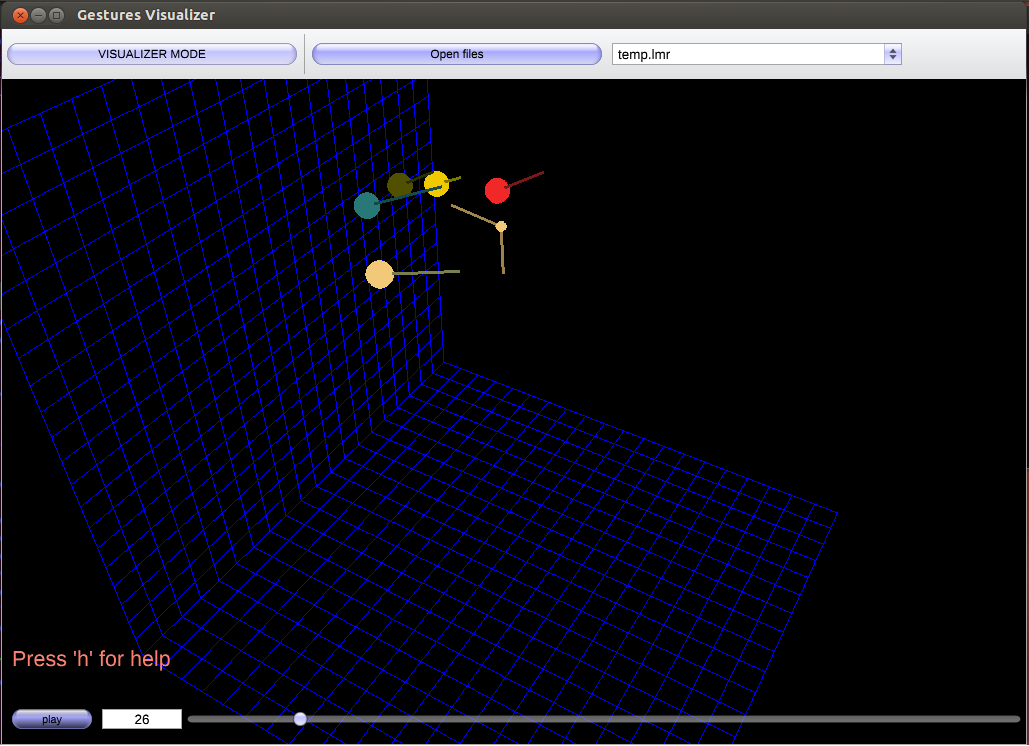
\includegraphics[width=1\columnwidth]{figures/visualizer.png}
 \caption{Screenshot of the visualizer}
 \label{visualizer}
\end{figure}

An example of parameter, which is not visualized, is finger width, in order not to obscure the image.
\begin{itemize}
\item Program can read the lmr files chosen by the user.
\item The user can load many files at once and select one of the recordings from the drop-down list.
\item To facilitate the user work with visualizer, program has implemented windowing interface.
\item The user has ability to rotate and zoom camera.
\item Slider is available in order to move between frames of the recording.
\item Visualizer has option to play recorded gesture, which the user can turn on and off by pressing the play/stop button.
\item There is also a button to enter the recorder mode.
\end{itemize}

\subsection{Recorder}
Recorder is part of the described module, which is responsible for collecting information from Leap Motion Controller and saving it to lmr file.
Each frame read from the Leap Motion is captured, and then converted to the previously described model. Then the model is saved by the appropriate sub-module to LMR file. The conversion process contains also sorting hands and fingers. Hands are sorted by X coordinate of palmPosition. In the case of sorting fingers, the usual sort by X coordinate is not enough. The order of the fingers must be independent from hand rotation, therefore a different method for fingers sorting had to be proposed. Fingers are sorted by distance between finger tip position and plane, which is perpendicular to the surface of the hand and contains a direction vector of a hand. This plane can be determined using palm position, direction vector and normalized normal vector of the hand.
Below is the formula for the distance ($d$) between finger tip position and designated plane.

\[ d = -(f - pp) \cdot (\hat{hd} \times \hat{hn}) \]
Where:
\begin{itemize}
    \item[] $f$: is the finger tip position
    \item[] $pp$: is the palm position
    \item[] $hd$: is the hand direction vector
    \item[] $hn$: is the hand normal vector
\end{itemize}

List of Recorder features:
\begin{itemize}
\item Turning on and off recording is done by using space key.
\item After recording window automatically appears, in which can be choosen where to save the file.
\item The recorder cooperates with the visualizer. During recording performed gesture is visualized.
\item There is a button to enter the visualizer mode.
\end{itemize}

\begin{figure}[htb]
\centering
 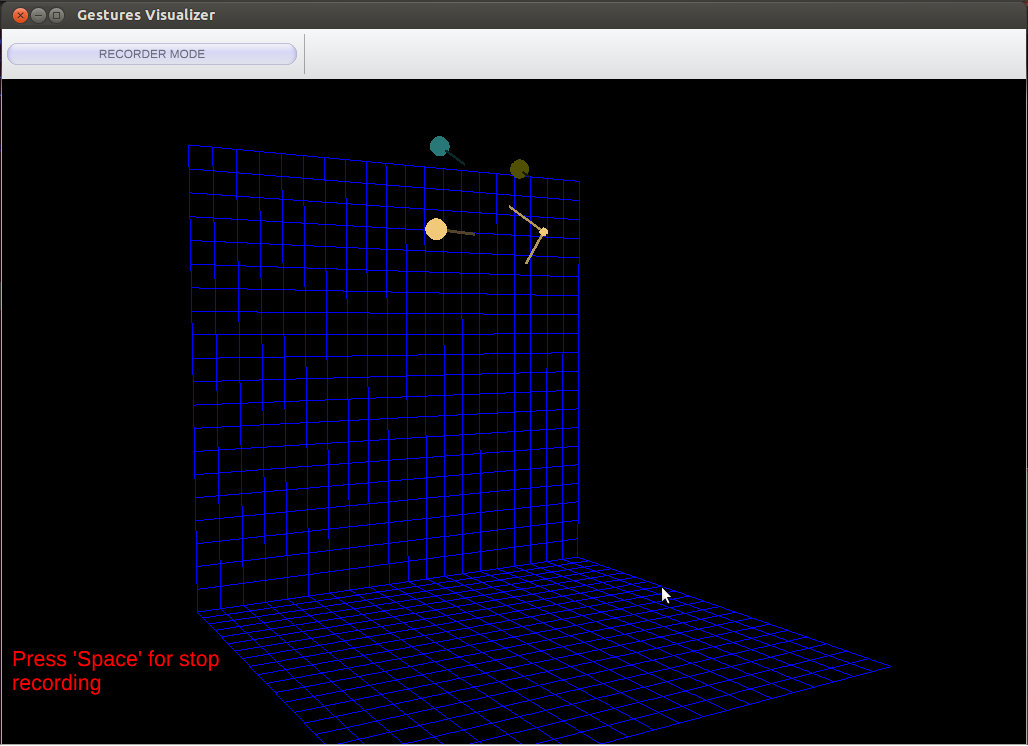
\includegraphics[width=1\columnwidth]{figures/recorder.png}
 \caption{Screenshot of the recorder}
 \label{recorder}
\end{figure}

\section{Used libraries}

\section{Samples of code using the library dedicated to Leap Motion Controller}
